\chapter{Results}
\label{chap:res}
In this section we will present and discuss the results from the experiments on the REST implementation. The experiments were conducted on an Intel(R) Xeon(R) Gold 6426Y processor with 500 GB RAM.

The dataset used for these experiments is distributed by \textcite{porto} and consists of taxi routes in the city Porto over the course of one year. These routes are in the form of trajectories with latitude longitude points. In total there are 1.7M trajectories, for most experiments 100K are used, otherwise this will be explicitly stated. 100K is used in order to achieve a feasible runtime, however the methods applied can also be used for larger dataset.

\section{Reference Set Construction}
Firstly we will look at reference set construction, both in terms of performance and set size. The metrics \textit{Sample size} and \textit{Set size} is the sample size used to construct the reference set and resulting set size. \textit{REST} is the implementation of the original algorithm, while \textit{REST-SF} is the same implementation with a spatial filter. The window size is also indicated in the name, following SF. \textit{REST-SF30} indicates the square's side length in the range query in meters. A window size of 30 means a box of $30\times30m^2$ for r-tree range queries.

\begin{figure}[ht]
    \begin{minipage}[b]{0.99\linewidth}
        \centering
        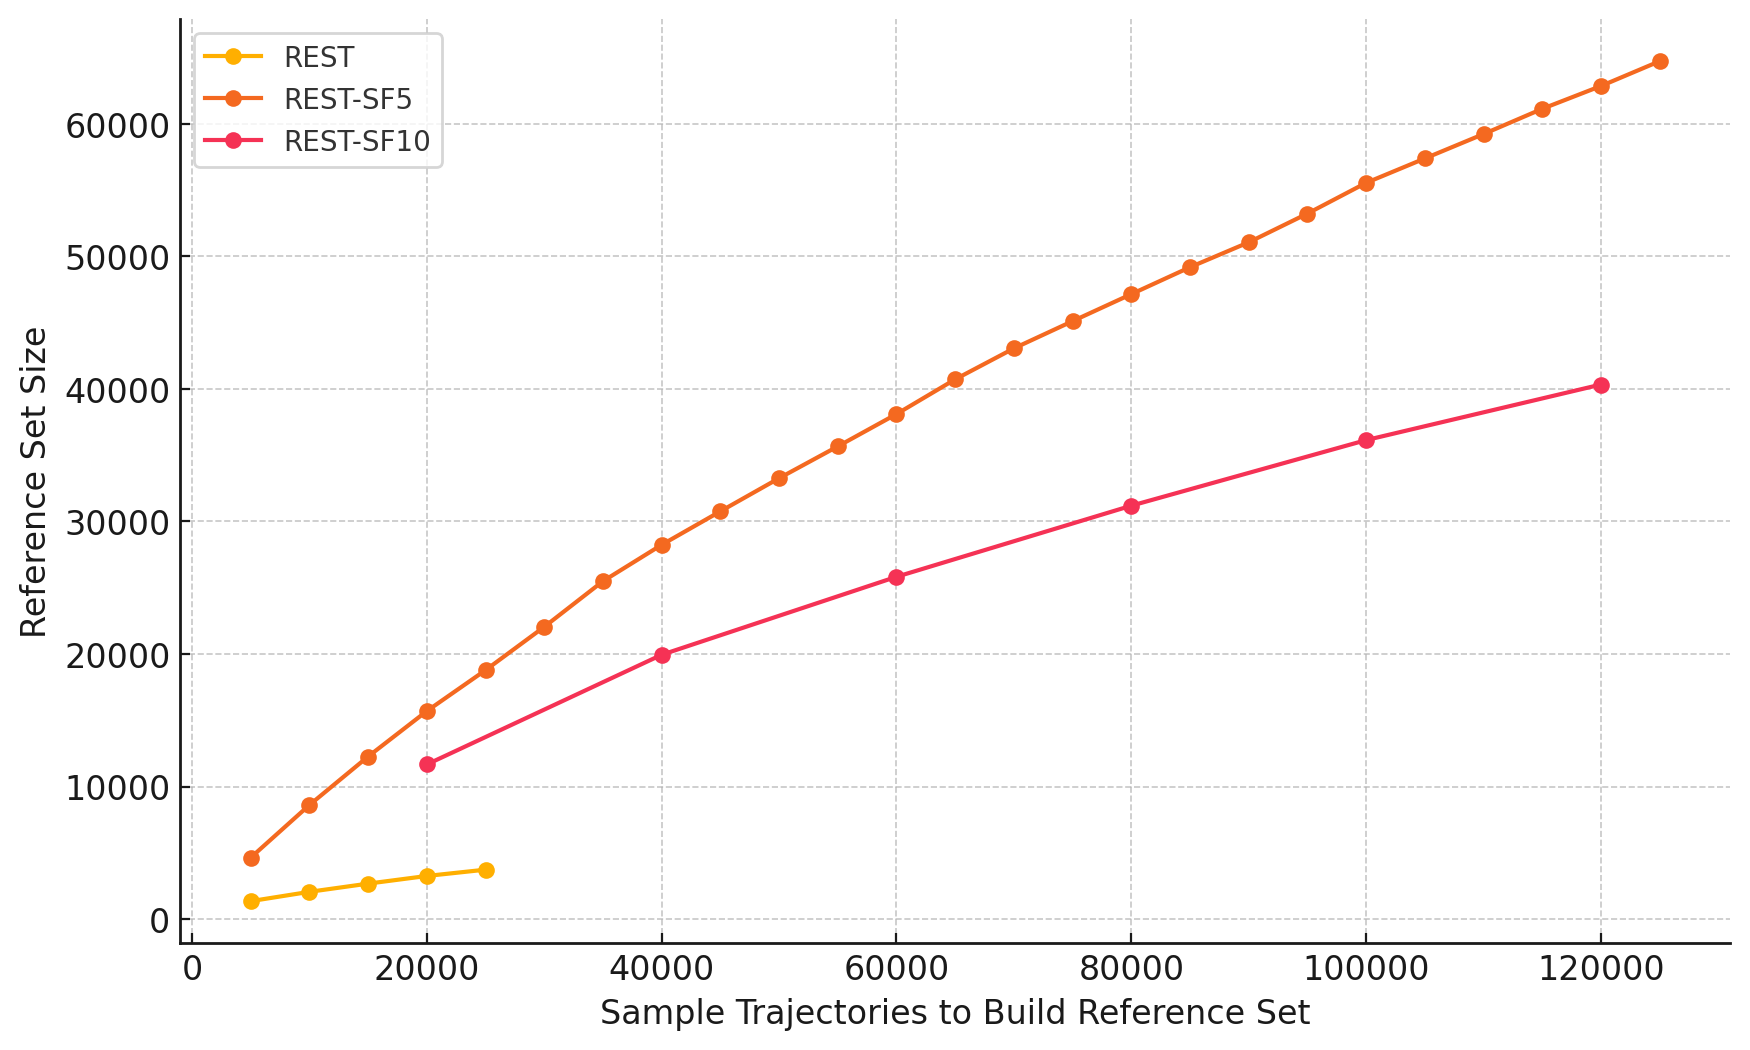
\includegraphics[height=8cm, keepaspectratio]{./figures/set_size.png}
        \caption{Reference set size over sample size. Each mode has a unique color}
        \label{fig:set_size}
    \end{minipage}
\end{figure}
\begin{figure}[h!]
    \begin{minipage}[b]{0.99\linewidth}
        \centering
        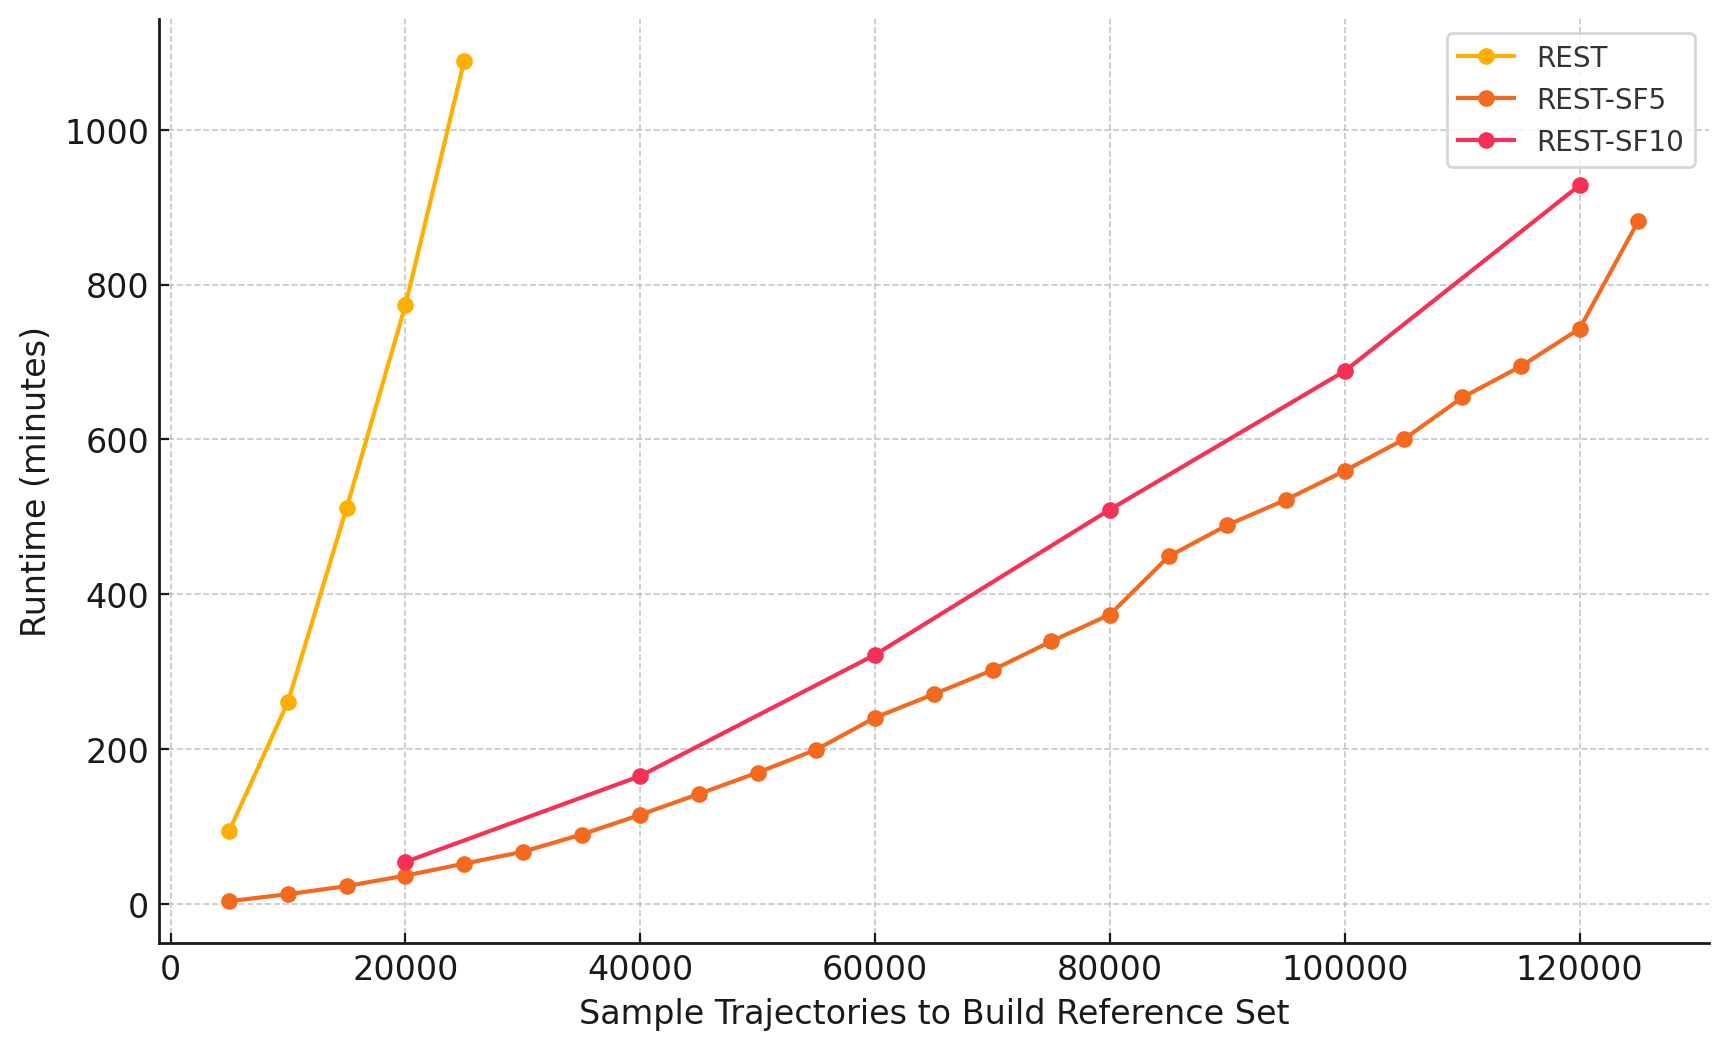
\includegraphics[height=8cm, keepaspectratio]{./figures/set_runtime.png}
        \caption{Reference set construction runtime over sample size. Each mode has a unique color}
        \label{fig:set_runtime}
    \end{minipage}
\end{figure}

In figure \ref{fig:set_size} we can see that \textit{REST} has a lower set size to sample size ratio, meaning it can represent a large sample with a small set. This must be considered the lower bound for sample size, since \textit{REST} can be seen as having an infinite window size, because it uses all reference trajectories. There is a trend that increasing window size approaches decreases set size, as we can see \textit{REST-SF75} is much lower in this regard than \textit{REST-SF15}. We also see that for all variants the growth in set size slowly decreases as sample size increases, this trend is also strongest for \textit{REST} closely followed by \textit{REST-SF75}. This might indicate the reference set size is approaching some finite value (converging) as the sample size increases. If the value converges, it makes a strong case for the effectiveness of reference based compression strategies in general. Intuitively this can be seen as the road network of a given city. If all the roads / routes have been mapped by the reference set then all new routes can also be represented by that.

For the runtime seen in \ref{fig:set_runtime} it is clear that \textit{REST} is much slower than the spatial filter variants. This is expected as it operates as if having an infinte window size, while \textit{REST-SF75} uses a $75\times75m^2$ window, significantly reducing the search space. There is a clear trend that increasing window size leads to increasing runtime. All in all, \textit{REST-SF75} seems to strike a balance between efficiency and maintaing a low sample size.
\section{Compression Performance}

\begin{figure}[ht]
    \begin{minipage}{0.99\linewidth}
        \centering
        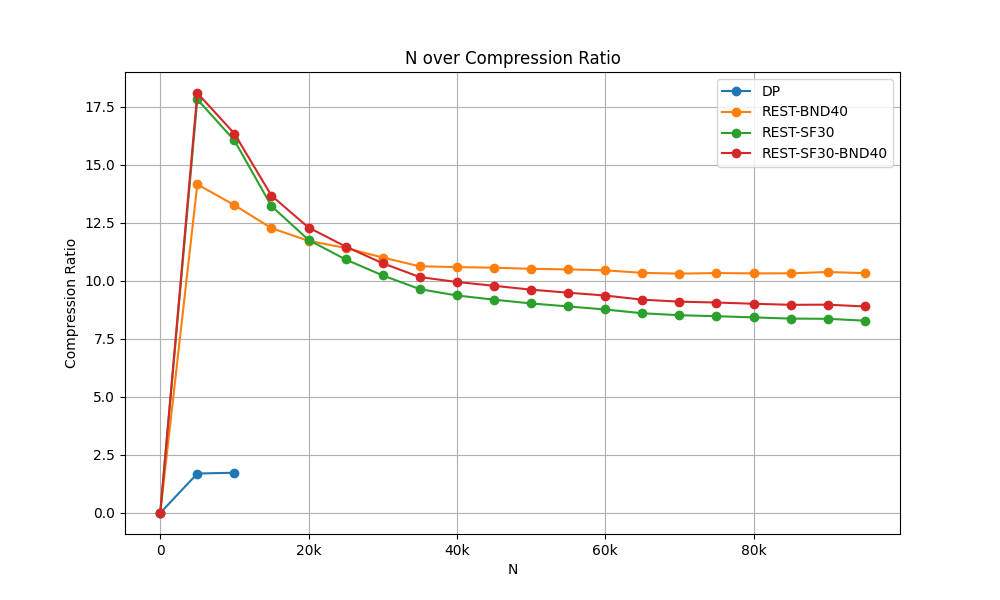
\includegraphics[height=8cm, keepaspectratio]{./figures/n_compression.png}
        \caption{N over compression ratio for a set sample size of 10k.}
        \label{fig:n_compression}
    \end{minipage}
\end{figure}
\begin{figure}[h!]
    \begin{minipage}{0.99\linewidth}
        \centering
        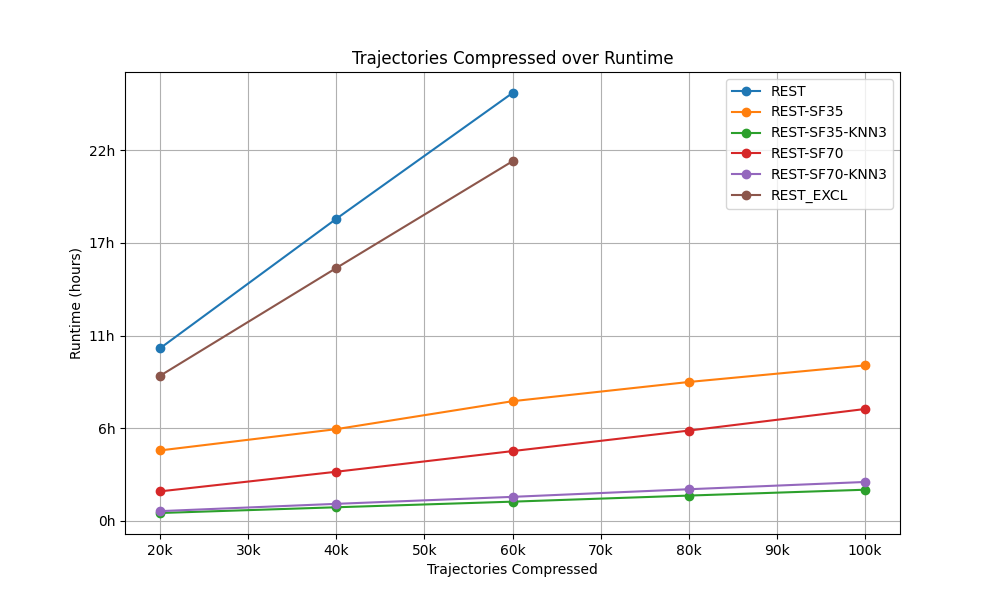
\includegraphics[height=8cm, keepaspectratio]{./figures/n_runtime.png}
        \caption{N over compression runtime, includes runtime for set construction with a sample size of 10k}
        \label{fig:n_runtime}
    \end{minipage}
\end{figure}
This section discusses the performance of the compression, using a reference set built from a sample size of 10k. $N$ represents the amount of compressed trajectories. Additionally we include experiments with the Sakoe-Chiba band, represented by BND in the graph label. The label \textit{REST-SF30-BND40} refers to a REST implementation that uses a spatial filter with a window size of 30 and a Sakoe-Chiba band size of 40. We also compare the different REST variants with Douglas-Peucker (DP). Figure \ref{fig:n_compression} show a clear spike in compression ratio at N = 10k for the REST variants. This is because many of the trajectories in the first 10k were added to the reference set and will have an exceptionally high compression ratio. Afterwards the compression ratio gradually falls, but stabilizes between 7.5-10.0. The compression ratio of DP is much lower, staying around a compression ratio of 2. The graph is cut off, however DP is expected to stay at the same level as N increases. this shows that REST significantly outperform DP.

However, note that the compression ratio for REST does not include the reference set size (this might change in future versions). This means that the real compression ratio will be lower, however considering the small size of the reference set compared to $N$, this is expected show promising results nonetheless.

With regards to runtime as seen in figure \ref{fig:n_runtime}, we see that all REST variations significantly outperform DP. When comparing REST variants we see that \textit{REST-SF30} is much faster than \textit{REST-BND40}. The combination of both strategies \textit{REST-SF30-BND40} only marginally outperforms \textit{REST-SF30}. This suggests that the spatial filter is most efficient speed up strategy, while the band only slightly improves performance. Looking at the differences between the two this indicates a bottle-neck for performance in REST. The spatial filter reduces the number of trajectory comparisons required, while the band decreases the runtime of each individual comparison. Thus, reducing the number of Dynamic Time Warping (DTW) distance calculations is a more efficient than speeding up individual calculations.